\documentclass{article}
\usepackage{nips12submit_e,times}
\usepackage{tikz}
\tikzstyle{vertex}=[auto=left,circle,fill=black!25,minimum size=20pt,inner sep=0pt]
\usepackage{verbatim}
\usepackage{url}
\usepackage{graphicx, color}
\usepackage{amsmath}
\usepackage{subfigure}

\title{Stochastic Blockmodels for Relational Event Data} 

\author{
David S.~Hippocampus\thanks{ Use footnote for providing further information
about author (webpage, alternative address)---\emph{not} for acknowledging
funding agencies.} \\
Department of Computer Science\\
Cranberry-Lemon University\\
Pittsburgh, PA 15213 \\
\texttt{hippo@cs.cranberry-lemon.edu} \\
\And
Coauthor \\
Affiliation \\
Address \\
\texttt{email} \\
\AND
Coauthor \\
Affiliation \\
Address \\
}


\begin{document} 

\maketitle

\begin{abstract}
Observing network data as a stream of events provides an opportunity to understand differences in how nodes behave given the past.  Recent methods for continuous-time network data model the rate of dyadic events conditioned on the observed history of events and covariates about the nodes.  Methods for static networks, such as stochastic blockmodels, often account for node-level heterogeneity by assuming latent groups of individuals have similar tendencies in their group-wise interactions.  We propose to combine these two approaches by modeling the event dynamics within and between clusters of nodes.  The method is illustrated using dyadic interaction data -- e.g. email, Twitter direct messages.  We show parameter estimates from the model reveal heterogeneity in the dynamics among groups of individuals.  The fitted models have better predictive accuracy than both baselines and relational event models without the latent structure.  Our approach illustrates the efficacy of combining a detailed model for local dependencies and a latent variable model for meso-scale dependencies.
\end{abstract}

\section{Introduction}

Statistical methods for analyzing network data have become increasingly useful for studying  phenomenon ranging from people communicating online to protein interactions \cite{Goldenberg2009}.  One class of statistical models for network data uses latent variables to help model unobserved heterogeneity.  For example, the stochastic blockmodel \cite{Nowicki2001, Kemp} assumes each node in the network belongs to some block (or cluster) and parametrizes the probability of edges between nodes of each block.  % Such approaches are especially useful for large-scale network data where higher-order dependencies can cause models such as exponential random graph models to be too complex to fit.

Network data, however, is often collected as a sequence of events occurring over time.   Recently work leverages  continuous time models from event history analysis  \cite{AalenOddO.2008} to model network-based event data \cite{Butts2008,Brandes2009,Perry2011,Stadtfeld2010,Stadtfeld2011,Opsahl2011,Vu2011,Vu2011a}.  These models allow one to specify how the process depends on the previous history of events.  In this way one may investigate theories about the underlying processes and make predictions about future data conditioned on the past.

The above continuous time network models assume all nodes in the network behave according to identical dynamics.  In many cases this is unrealistic.  For example, in a small organization comprised of several teams, each team may exhibit different patterns for collaborating via email --  individuals in one group may respond more quickly, while another group may preferentially send to highly active individuals.  %, and in many cases emails between one pair of individuals will not affect emailing behavior between a separate pair of individuals.

Borrowing from the intuition of stochastic blockmodels, we propose a hierarchical model of continuous time network data that assumes latent clusters of nodes share similar patterns of interaction.  The behavior of the model is illustrated with simulated data.  We describe parameter estimation and the learning of the latent cluster assignments via MCMC.  Using data sets of dyadic communication among people, we compare the predictive performance of the fitted models to standard baselines.  Finally we show that the parameter estimates exhibit an interpretable structure to the event dynamics, sometimes identifying particular \emph{roles} of communication.
  
\section{Model}

%Each interaction then has a set of periods $d \in D_{ij}$ each with a start time $a_d$, an end time $b_d$, and a rate $\lambda_d$.
Consider a nonhomogeneous Poisson process with  intensity $\lambda(t)$ that is piecewise constant with respect to a set of knots $\tau$.  We can then write the likelihood of $M$ events as
\begin{align}
\mathcal{L}(\mathcal{A}|\theta) &= \prod_{m=1}^M \lambda(t_m) \exp\left\{ - \int_{0}^{t_M} \lambda(s)ds \right\} \\
&= \prod_{m=1}^M \lambda(t_m) \prod_{k=1}^{|\tau|} \exp\left\{ - (\tau_{k} - \tau_{k-1}) \lambda(\tau_k) \right\}
\end{align}
\noindent where the $m$th event occurs at time $t_m$, the intensity function $\lambda(t)$ is left continuous, and each $\tau_k \in [0,t_M]$.
% \begin{align}
% \mathcal{L}(A|\theta) &= \prod_{m=1}^M \lambda_{i_m}(t_m|\cdot) \prod_{i \in \mathcal{R}}  \exp\left\{ - \int_{0}^{t_M} \lambda_{i}(\tau | \cdot)d\tau \right\} \\
% &= \prod_{m=1}^M \lambda_{i_m}(t_m|\cdot) \prod_{i \in \mathcal{R}} \prod_{v \in D_{i}} \exp\left\{ - (b_v - a_v) \lambda_{i}(b_v | \cdot ) \right\}
% \end{align}

One can extend the above to marked point processes where each event contains additional information.  In the context of relational events occurring among $N$ nodes, each event in the process contains both a sender $i$ and a recipient $j$ such that  $(i,j) \in \mathcal{R}$, where $\mathcal{R}$ is the \emph{risk set} comprised of all allowed dyads.  We assume each dyad $(i,j) \in \mathcal{R}$ occurs as a Poisson process with intensity $\lambda_{ij}(t)$ that is piecewise constant.  We can then write the likelihood as  
\begin{align}
\mathcal{L}(\mathcal{A}|\theta) &= \prod_{m=1}^M \lambda_{i_m,j_m}(t_m|\cdot) \prod_{(i,j) \in \mathcal{R}_{i_m,j_m}}\exp\{ - (t_m - \tau_{mij}) \lambda_{ij}(t_m | z_i,z_j) \}
\label{eqn:llk}
\end{align}
\noindent where event $m$ is the dyad $(i_m,j_m)$, $\tau_{mij}$ is the time  of the changepoint for $\lambda_{i,j}$ prior to the $m$th event, and $\mathcal{R}_{i,j}$ is the set of dyads whose intensity changes if $(i,j)$ occurs. \footnote{We further assume 1) all intensity functions change at times $t=0$ and $t=t_M$, and 2) the first event is drawn uniformly from the risk set.}

\begin{figure}

\centering 
\subfigure[Dynamic network data]
{
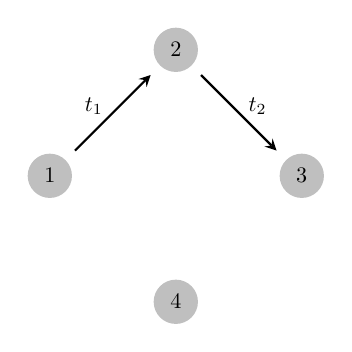
\begin{tikzpicture}[scale=.8,transform shape,thick]
  \node[vertex] (n1) at (0,0)  {1};
  \node[vertex] (n2) at (2,2)  {2};
  \node[vertex] (n3) at (4,0) {3};
  \node[vertex] (n4) at (2,-2) {4};
\draw[-stealth] (.4,.4) -- (1.6,1.6);
\draw[-stealth] (2.4,1.6) -- (3.6,.4);
\node at (.7,1.1) {$t_1$};
\node at (3.3,1.1) {$t_2$};
\end{tikzpicture}
}
\subfigure[Intensities for two dyads]
{
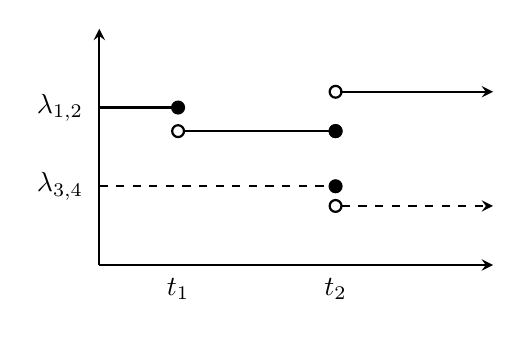
\begin{tikzpicture}[scale=1,transform shape,thick]
\draw[-stealth] (0,0) -- (0,3);
\draw[-stealth] (0,0) -- (5,0);

% First timeline
\draw (0,2) -- (1,2);
\draw[fill=black] (1,2) circle (0.75mm);
\draw (1,1.7) circle (0.75mm);
\draw (1.08,1.7) -- (3,1.7);
\draw[fill=black] (3,1.7) circle (0.75mm);
\draw (3,1.7) circle (0.75mm);
\draw (3,2.2) circle (0.75mm);
\draw[-stealth] (3.05,2.2) -- (5,2.2);

% second timeline
\draw[dashed] (0,1) -- (3,1);
\draw[fill=black] (3,1) circle (0.75mm);
\draw (3,.75) circle (0.75mm);
\draw[dashed, -stealth] (3.08,.75) -- (5,.75);

% labels
\node at (-.5,2) {$\lambda_{1,2}$};
\node at (-.5,1) {$\lambda_{3,4}$};
\node at (1,-.3) {$t_1$};
\node at (3,-.3) {$t_2$};
\end{tikzpicture}
}
\caption[]{Illustration of event data and the assumptions of the model.  Left: An sequence of two events among four nodes: (1,2) occurs at time $t_1$ and (2,3) occurs at time $t_2$.  Right: The intensity functions $\lambda_{1,2}(t)$ (solid) and $\lambda_{34}(t)$ (dotted).  Note $\lambda_{34}$ can only change when events occur that involve either node 3 or node 4.\footnotemark }
\label{fig:example}
\end{figure}

\footnotetext{TODO? Illustration of the block model, where events in cluster 1 (circles) are governed by the vector $\beta_{1,1}$, events in cluster 2 (squares) are governed by $\beta_{2,2}$, and an circle-to-square event governed by $\beta_{1,2}$.}


% \begin{figure}
%  \def\svgwidth{6in}
%   \input{example1.pdf_tex}
% \caption{Illustration of event data and the assumptions of the model.  Left: An sequence of two events among four nodes: (1,2) occurs at time $t_1$ and (2,3) occurs at time $t_2$.  Center: The intensity functions $\lambda_{1,2}(t)$ (solid) and $\lambda_{34}(t)$ (dotted).  Note $\lambda_{34}$ can only change when events occur involving either node 3 or node 4.  Right: Illustration of the block model, where events in cluster 1 (circles) are governed by the vector $\beta_{1,1}$, events in cluster 2 (squares) are governed by $\beta_{2,2}$, and an circle-to-square event governed by $\beta_{1,2}$.}
% \label{fig:example}
% %\includegraphics[width=6in]{example}
% \end{figure}

For a given dyad $(i,j)$ and time $t$ we may also have a vector of statistics $\mathbf{s}(t,i,j|\mathcal{A}_t,\mathbf{z})$ that is a function of the previous event history  $\mathcal{A}_t = \{(t_m,i_m,j_m): t_m \in [0,t)\}$.   In practice we may believe an interaction between one dyad should not affect the rate of an entirely separate dyad.  As shown in Figure \ref{fig:example}, we incorporate this idea by assuming each intensity function $\lambda_{ij}(t)$ may only change following an event involving either $i$ or $j$.  This implies that  $\mathcal{R}_{i,j}$ is the set of dyads involving either $i$ or $j$ and that we will only use  statistics $\mathbf{s}(t,i,j)$ that do not change until an event involving either $i$ or $j$ occurs.  

We hope to learn about the dynamics between subsets of nodes.   To facilitate this, we assume node $i$ is assigned a latent cluster $z_i$ and the intensity functions via a log linear model
\begin{align*}
\log \lambda_{ij}(t | \mathcal{A}_t,\mathbf{z}) &= \boldsymbol{\beta}_{z_i,z_j} \mathbf{s}(t,i,j|\mathcal{A}_t) &
z_i &\sim \mbox{CRP}(\alpha) &
\beta_{k,l,p} &\sim \mbox{N}(\mu_p,\sigma_p^2)
\end{align*}
where for each pair of clusters $(z_i,z_j)$ we have a vector of parameters $\boldsymbol{\beta}_{z_i,z_j}$ that corresponds to the vector of statistics $\mathbf{s}(t,i,j|\cdot)$.   Thus, the model of dynamics for the dyad $(i,j)$ has the same parameters as for other dyads occurring between group $z_i$ and $z_j$.  We allow  the blocks to share information by placing a hierarchical prior on the collection of $\boldsymbol{\beta}_{k.l}$.

\subsection{Model specification}
  
% \begin{enumerate}
% \item Intercept: $s_{0}(t,i,j) = 1$
% \item Dyad count: $s_{1}(t,i,j) = f(\sum_{m:t_m<t} I(i_m=i) )$
% \item Sender out-degree: $s_{1}(t,i,j) = f(\sum_{m:t_m<t} I(i_m=i) )$
% \item Sender in-degree: $s_{2}(t,i,j) = f(\sum_{m:t_m<t} I(j_m=i) )$
% \item Receiver out-degree: $s_{3}(t,i,j) = f(\sum_{m:t_m<t} I(i_m=j))$
% \item Receiver in-degree: $s_{4}(t,i,j) = f(\sum_{m:t_m<t} I(j_m=j))$
% \item Reciprocity (AB-BA): $s_{5}(t,i,j) = I(i_m=i,j_m=j,i_{v_{mij}}=j,j_{v_{mij}}=i)$
% \item Turn-taking (AB-BY): $s_{6}(t,i,j) = I(i_m=i,j_m=j,i_{v_{mij}}=j,j_{v_{mij}}=i)$
% \item Turn-usurping (AB-XA): $s_{7}(t,i,j) = I(i_m=i,j_m=j,i_{v_{mij}}=j,j_{v_{mij}}=i)$
% \item Turn-usurping (AB-XB): $s_{8}(t,i,j) = I(i_m=i,j_m=j,i_{v_{mij}}=j,j_{v_{mij}}=i)$
% \item Turn-continuing (AB-AY): $s_{9}(t,i,j) =  I(i_m=i,j_m=j,i_{v_{mij}}=j,j_{v_{mij}}=i)$
% %\item Number of shared two-paths: $s_{10}(t,i,j) =   \sum_{m:t_m<t} \sum_{r=1}^NI(i_m=i,j_m=r or i_m=r,j_m=j)$
% % \item Shared contacts (since last occurrence): $s_{ij10}(t,i,j) = \sum_{r=1}^N I(i_m=i,j_m=j,i_{v_{mij}}=i,j_{v_{mij}}=r)$
% % \item Triadic closure (since last occurrence): $s_{ij11}(t,i,j) = \sum_{r=1}^N I(i_m=i,j_m=j,i_{v_{mij}}=r,j_{v_{mij}}=j)$
% % \item Shared contacts (since last occurrence): $s_{ij12}(t,i,j) = \sum_{r=1}^N I(i_m=i,j_m=j,i_{v_{mij}}=r,j_{v_{mij}}=r)$
% \end{enumerate}

\begin{table}[t]
\footnotesize
\center
\begin{tabular}{|l|l|}
\hline
Statistic & Formula \\
\hline
\hline
Intercept& $s_{0}(t,i,j) = 1$\\
Dyad count& $s_{1}(t,i,j) = f(\sum_{m:t_m<t} I(i_m=i,j_m=j) )$\\
Sender out-degree& $s_{1}(t,i,j) = f(\sum_{m:t_m<t} I(i_m=i) )$\\
Sender in-degree& $s_{2}(t,i,j) = f(\sum_{m:t_m<t} I(j_m=i) )$\\
Receiver out-degree& $s_{3}(t,i,j) = f(\sum_{m:t_m<t} I(i_m=j))$\\
Receiver in-degree& $s_{4}(t,i,j) = f(\sum_{m:t_m<t} I(j_m=j))$\\
Reciprocity (AB-BA)& $s_{5}(t,i,j) = I(i_m=i,j_m=j,i_{v_{mij}}=j,j_{v_{mij}}=i)$\\
Turn-taking (AB-BY)&$s_{6}(t,i,j) = I(i_m=i,j_m=j,i_{v_{mij}}=j,j_{v_{mij}}\ne i)$\\
Turn-usurping (AB-XA)& $s_{7}(t,i,j) = I(i_m=i,j_m=j,i_{v_{mij}} \ne j,j_{v_{mij}}=i)$\\
Turn-usurping (AB-XB)&$s_{8}(t,i,j) = I(i_m=i,j_m=j,i_{v_{mij}} \ne i,j_{v_{mij}}=j)$\\
Turn-continuing (AB-AY)& $s_{9}(t,i,j) =  I(i_m=i,j_m=j,i_{v_{mij}}=i,j_{v_{mij}}\ne j)$\\
\hline
\end{tabular}
\label{tab:stats}
\caption{Statistics used to specify intensity functions using the previous history $\mathcal{A}_t$.}
\end{table}



In Table \ref{tab:stats} we list the statistics we use in our experiments for  $\mathbf{s}(t,i,j)$.  Several statistics use $v_{mij} \in [0,M]$, the index of the last event where $(i,j)$ occurred (n.b. $t_{v_{mij}} = \tau_{mij}$). If $(i,j)$ has never occurred, we set $v_{mij}=0$.  Here we include degree effects to model possible rich-get-richer phenomenon.  For example, a particular node sending often may indicate they will continue to be a sender in the future.  We normalize these counts by the number of events up until a dyad's prior changepoint.\footnote{This seems to avoid ``explosion'' when simulating from the model.  TODO: Explore the theory about these sorts of statistics.  Aalen has a few suggestions.} Other statistics could be of interest for particular substantive questions \cite{Butts2008,Vu2011}.  \footnote{Describe the form of $f()$.  Right now it is $f(x) = \log \frac{x+1}{m + N(N-1)}$.}

The next set of statistics are \emph{participation shift} effects inspired by research in conversational norms \cite{Gibson2003}.  For example, an AB-BA effect indicates an increased propensity for reciprocity.  The final set of effects allow one to model phenomenon such as triadic closure.  Though we use only the above statistics in our experiments, one may use any quantity or set of covariates about a given dyad that is computed using the previous history of events.  The only restriction is that the statistic may not change in value between each observed event.\footnote{This prevents one from using the number of events occurring in some previous time window, as in \cite{Gunawardana2011}.}

\subsection{Relation to other models}

Our formulation is reminiscent of the stochastic blockmodel \cite{Nowicki2001,Kemp} which models the probability of a dyad as $p(y_{ij}) =\mbox{logit}^{-1}( \eta_{z_i,z_j})$ where $\eta_{z_i,z_j}$ is interpreted as a mixing rate between group $z_i$ and group $z_j$.  In the proposed method, however, the blockmodel structure facilitates the study of intra-group and inter-group dynamics via a continuous-time network model.

The above framework generalizes several important special cases. For example,  using only the intercept statistic $s_0(t,i,j) = 1$ is analogous to the stochastic block model for static networks.  Under this model each dyad is a homogeneous Poisson process and all dyad intensities $\lambda_{i,j}$ within block $(z_i,z_j)$ have the same intensity, $\exp\{\boldsymbol{\beta}_{z_i,z_j}\}$.  As these intensities do not change under this specification, the likelihood simplifies to 
$$\mathcal{L}(\mathcal{A}|\beta) = \prod_{m=1}^M \lambda_{i_m,j_m} \prod_{(i,j) \in \mathcal{R}} \exp\{-t_M \lambda_{i,j}\}$$

Alternatively, if one models only the order of the events (ignoring the times at which they occur), the likelihood can be written as
\begin{align}
\mathcal{L}_{\mbox{mult}}(\mathcal{A}|\beta) = \prod_{m=1}^M \frac{\lambda_{i_m,j_m}(t_m | \cdot)}{\sum_{(i,j) \in \mathcal{R}} \lambda_{i,j}(t_m | \cdot)}.
\label{eqn:multllk}
\end{align}
The functional form is similar to conditional logit models used for discrete choice data \cite{McFadden1984}, though here the possible choices are all the dyads in $\mathcal{R}$.


\section{Inference}

We use Markov chain Monte Carlo to sample from the posterior distribution of our parameters.  

\subsection*{Sampling $\mathbf{z}$ given $\boldsymbol{\beta}$ and $\mathcal{A}$ }

We Gibbs sample the latent class assignments $\mathbf{z}$ from the conditional distribution
\begin{align*}
p(z_i | z_{-i},\mathcal{A},\alpha,\boldsymbol{\beta}) &\propto p(z_i | z_{-i},\alpha) p(\mathcal{A}|\mathbf{z},\boldsymbol{\beta},\mbox{node} \ i \ \mbox{involved}) \\
p(\mathcal{A}|\mathbf{z},\boldsymbol{\beta},\mbox{node} \ r \ \mbox{involved}) &= \prod_{a \in \mathcal{U}_r} \lambda_{i_a,j_a}(t_a|\cdot)
\prod_{(i,j) \in \mathcal{R}_{i_a,j_a}} \exp \{ -(t_a - \tau_{aij}) \lambda_{ij}(t_a|\cdot)\}
\end{align*}
where $\mathcal{U}_r = \{a: r \in \{i_a,j_a\}, a \in [1,M]\}$ is the set of events where node $r$ is involved.  Under a CRP($\alpha$) prior, we have $p(z_i = k | z_{-i},\alpha) = n_k $ and $p(z_i = \mbox{new} |  z_{-i},\alpha) = \alpha$ where $n_k$ is the number of nodes assigned to cluster $k$. 
% \begin{align*}
% p(z_i = k | z_{-i},\alpha) &= n_k & p(z_i = \mbox{new} |  z_{-i},\alpha) &= \alpha
% \end{align*}


 By limiting the changepoints to times when either node is involved, computing the likelihood $p(A|z,\beta,\mbox{node} \ r \ \mbox{involved})$ is $O(|\mathcal{U}_r| \cdot P \cdot 4N)$.  The factor of 4 is due to the number of dyads involving a single node.  We precompute $\tau_{m,i,j}$ and $\mathbf{s}(t_m,i,j)$ for all $m,i,j$. 


\subsection{Sampling $\boldsymbol{\beta}$ given $\mathbf{z}$ and $\mathcal{A}$ }

For each block $(k,l)$ we need to sample the vector of parameters $\boldsymbol{\beta}_{k,l}$ from its posterior
\begin{align*}
p(\boldsymbol{\beta}_{k,l} | \mathcal{A}_t, \textbf{z}, \mu, \sigma) &\propto p(\boldsymbol{\beta}_{k,l} | \mu, \sigma) p( \mathcal{A}| \textbf{z}, \boldsymbol{\beta}, \mbox{cluster} \ k \ \mbox{or} \ l \ \mbox{involved}) \\  
p(\boldsymbol{\beta}_{k,l} | \mu, \sigma) &= \prod_{p=1}^Pp(\beta_{k,l,p}|\mu_p,\sigma_p^2)\\
p(\mathcal{A}|\mathbf{z},\boldsymbol{\beta}, \mbox{cluster} \ k \ \mbox{or} \ l \ \mbox{involved}) &= \prod_{a \in \mathcal{U}_r} \lambda_{i_a,j_a}(t_a|\cdot)
\prod_{(i,j) \in \mathcal{R}_{i_a,j_a}} \exp \{ -(t_a - \tau_{aij}) \lambda_{ij}(t_a|\cdot)\}
\end{align*}
where $\mathcal{V}_{k,l} = \{a: z_{i_a} \in \{k,l\} \ \mbox{or} \ z_{j_a} \in \{k,l\}, a \in [1,M]\}$ is the set of events $a$ where one of the nodes is either in block $k$ or $l$.  \footnote{TODO: If we end up using HMC, mention step size and step length used.}
This distribution is sampled using slice sampling.\footnote{We may also use HMC for this.}

\subsection{Split-merge algorithm}

Motivation: simply Gibbs sampling does not seem to mix well.  \footnote{This section is planned future work. In the experiments we evaluate the performance of the model when restricting the number of clusters $K$.  For these chains we do not propose split moves when the number of non-empty clusters is already $K$.}

IDEA: References are Dahl 2003, Wang, Blei 2012, Neal 2000 (alg 8).  A proposed split has REM parameters that are only slightly different than those for the original block.  Merges of two sets of REM parameters are performed by using the parameter for one blocks, and doing so for each dimension independently.  By keeping track of the probability of each of these transitions we can correctly compute the Metropolis-Hastings acceptance probability needed to guarantee we have an MCMC transition that leaves the posterior distribution invariant.

This is a two-stage MH procedure, first picking two nodes at random then creating a new set of parameters.  We also use an auxilary variable to avoid changing dimensionality (similar to Neal 2000, alg. 8).

%$\boldsymbol{\phi}_{l,r}^{split} \sim G_0$, $\boldsymbol{\phi}_{r,l}^{split} \sim G_0$, and $\boldsymbol{\phi}_{l,l}^{split} \sim G_0$ (or actually $N(\mu_{\phi},\Sigma_{\phi})$

Next pick two nodes $i,j$ uniformly.  If they belong to the same block $k$ (i.e. $z_i=z_j=k$), then we call the current state the ``merge'' state $(\boldsymbol{\phi}^{merge},\mathbf{z}^{merge}) = (\boldsymbol{\phi},\mathbf{z})$ and propose a ``split'' state $(\boldsymbol{\phi}^{split},\mathbf{z}^{split})$ by letting $l=K+1$ and for $p \in [1,P], r \in [1,K]$
\begin{itemize}
%\item For $p \in [1,P], r \in [1,K]$: let $l=K+1$ sample $\phi_{lrp}^{merge},\phi_{rlp}^{merge}$, and $\phi_{llp}^{merge}$ independently from the prior $N(\mu_p,\sigma^2_p)$
\item Sample $\phi_{lrp}^{split} \sim N(\phi_{krp}^{merge},\sigma^2)$ and $\phi_{rlp}^{split} \sim N(\phi_{rkp}^{merge},\sigma^2)$ and $\phi_{llp}^{split} \sim N(\phi_{kkp}^{merge}, \sigma^2)$.
\item Sample $\phi_{lrp}^{merge},\phi_{rlp}^{merge}$, and $\phi_{llp}^{merge}$ independently from the prior $N(\mu_p,\sigma^2_p)$.
\item Let $S$ be all nodes assigned to $k$.  Randomly assign $z_a^{split}$ and perform restricted Gibbs scan for $\mathbf{z}^{split}$: $$p(z_{a}^{split}=k|\cdot)  \propto m_k p(A|\mathbf{z}^{split}_{-a},\phi^{split})$$
where $m_k=\sum_{i \in S}I(z_i=k)$ and compute $q( \mathbf{z}^{merge} \rightarrow \mathbf{z}^{split})$ to be the product of the probabilities for the sampled assignments.
\item Accept  $(\boldsymbol{\phi}^{split},\mathbf{z}^{split})$ as the new state with probability $\alpha^*$, defined below.
\end{itemize}

  If $i$ and $j$ belong to different blocks $k$ and $l$ (i.e. $z_i = k \ne z_j=l$), we define the current state to be the ``split'' state  $(\boldsymbol{\phi}^{split},\mathbf{z}^{split}) = (\boldsymbol{\phi},\mathbf{z})$ and propose a ``merge'' state $(\boldsymbol{\phi}^{merge},\mathbf{z}^{merge})$ as follows:
\begin{itemize}
\item For each $p \in [1,P]$ and for all blocks $r \in [1,K], r\ne l$ draw $\phi_{krp}^{merge}$ uniformly from $\{\phi_{krp}^{split}, \phi_{lrp}^{split}\}$,  $\phi_{rkp}^{merge}$ uniformly from $\{\phi_{rkp}^{split}, \phi_{rlp}^{split}\}$
\item Sample $\phi_{lrp}^{split},\phi_{rlp}^{split}$, and $\phi_{llp}^{split}$ independently from the prior $N(\mu_p,\sigma^2_p)$
\item Let $S$ be the set of nodes assigned to $k$ or $l$. Let $\mathbf{z}$ be a random assignment for nodes a and compute the probability of sampling $\mathbf{z}^{split}$ during a restricted Gibbs scan as $q( \mathbf{z}^{merge} \rightarrow \mathbf{z}^{split}) = \prod_{s \in S} p(z_{s}=z_s^{split} |\{ z_a^{split},z_{b}: a  < s, s < b\}, \boldsymbol{\phi}^{split})$
\item Accept $(\boldsymbol{\phi}^{merge},\mathbf{z}^{merge})$ as the new state with probability $1/\alpha^*$, defined below.
\end{itemize}

The Metropolis-Hastings acceptance probability for the split move is: $$\alpha^* =\frac{p(\boldsymbol{\phi}^{split})}{p(\boldsymbol{\phi}^{merge})} \frac{p(\mathbf{z}^{split})}{p(\mathbf{z}^{merge})}\frac{p(A|\boldsymbol{\phi}^{split},\mathbf{z}^{split})}{p(A|\boldsymbol{\phi}^{merge},\mathbf{z}^{merge})}\frac{q(\mathbf{z}^{split} \rightarrow \mathbf{z}^{merge})}{q( \mathbf{z}^{merge} \rightarrow \mathbf{z}^{split})} \frac{q(\boldsymbol{\phi}^{split} \rightarrow \boldsymbol{\phi}^{merge})}{q(\boldsymbol{\phi}^{merge} \rightarrow \boldsymbol{\phi}^{split})}$$

The first two terms represent the prior. For the proposed merge step, note $q(\boldsymbol{\phi}^{split} \rightarrow \boldsymbol{\phi}^{merge}) = .5^{P(2K-3)}$ where $K$ is the number of blocks before the move.  We can compute $q(\boldsymbol{\phi}^{merge} \rightarrow \boldsymbol{\phi}^{split})$ directly as a product of Normal densities.  For the block assignments, $q(\mathbf{z}^{split} \rightarrow \mathbf{z}^{merge})=1$ since  there is only one way of combining two clusters.  $ \frac{p(\mathbf{z}^{split})}{p(\mathbf{z}^{merge})} = \frac{(n_{z_i}^{split} - 1)!(n_{z_j}^{split} - 1)!}{(n_{z_i}^{merge}-1)!}$.  We have avoided the dimensionality of the model during the MH move by creating an empty cluster when merging and filling a (newly created) empty cluster when splitting.  One can return to the previous state with positive probability.

% TODO: Update the following discussion about sampling.

% This operation can be done in parallel, and only the portion of the likelihood involving the newly assigned cluster  need to be recomputed.  Computing the likelihood is then $O(T \cdot P \cdot 4N)$ (though this computation is split into $K^2$ pieces) and must computed $N \cdot K$ times per Gibbs iteration.  The most straightforward implementation has space complexity $O(N^2)$ since we must keep track of $\tau_{i,j,m}$ for each $(i,j)$ at a given $m$.

% \subsection{Approximate likelihood methods}

% TODO: Discuss how one might sample the likelihood.  Cite Raftery paper.

% TODO: Look at performance of this with respect to bias and performance measure

\begin{figure}
\center
\includegraphics[width=1.6in]{../figs/synthetic/mat.pdf}
\includegraphics[width=2in]{../figs/synthetic/counts.pdf}
\includegraphics[width=1.8in]{../figs/synthetic/params-estimates.pdf}
\caption{Illustration of 2000 simulated events, as described in text. Left: Counts of each dyad. Center: Boxplot of distribution of participation counts across dyads.  The top left shows an increased propensity for reciprocity within cluster 1; bottom right shows more AB-AY events within cluster 2.  Right: Parameters (in red) and posterior credible intervals (in black).}
\label{fig:syncounts}
\end{figure}

\section{Simulation}

We check our model fitting procedure using a small synthetic data set involving 10 nodes from 2 clusters where 1) the first cluster has an increased tendency for reciprocity, 2) members of the second cluster have an increased tendency to continue speaking, and 3) interactions between groups are more likely to be repeated.  The specification of $\textbf{s}$ is therefore $s(t,i,j) = [s_0, s_{5}(t,i,j), s_{9}(t,i,j)]$.  For the synthetic data set we use parameter vectors $\boldsymbol{\beta}_{1,1} = (0,3,0)$,  $\boldsymbol{\beta}_{1,2} = \boldsymbol{\beta}_{2,1} = (-1,0,0)$, and $\boldsymbol{\beta}_{2,2} = (0,0,2)$.  This is done by sequentially computing $\lambda_{ij}(t_m|\cdot)$ for all $(i,j) \in \mathcal{R}$, drawing $t_{m+1}-t_m \sim \mbox{Exp}(\sum_{ij} \lambda_{ij}(t_m|\cdot))$, and drawing the dyad $(i,j) \sim \mbox{Categorical}(\lambda_{ij}(t_m|\cdot) / \sum_{ij}\lambda_{ij}(t_m|\cdot))$.  

Though the dyad counts for the synthetic data set suggest a stochastic blockmodel (as seen in Figure  \ref{fig:syncounts}),  the center plot shows each block has empirical differences in their dynamics.  Intensities for reciprocal actions among nodes in block 1 are $e^3$ times greater, intensities for turn-taking actions among nodes in group 2 are $e^2$ times greater, and intensities for dyadic interactions between the two groups have a multiplicative effect of $e^{-1}$ and thus occur less often.  Fitting the model with $K=2$ converges to the true loglikelihood (see Table \ref{tab:results}) and the posterior credible intervals of the parameters cover the true parameter values.

\section{Model checking and experiments}

\subsection{Data}

Each of the following data sets are sequences of dyadic events, where each event has a time associated with it, a sender, and a recipient.

\begin{itemize}
\item Kiel email: \cite{Ebel2002}
\item Enron email:
\item Tweets from Twitter.com occurring between from May 11, 2009 to January 26, 2012 that contained the hashtag \texttt{\#rstats}.\footnote{Will be made publicly available.}  This hashtag is used to denote messages pertaining to the R statistical computing environment and sometimes statistical discussion more generally.  We collect dyadic events by selecting tweets beginning with the \texttt{@} symbol (called a \emph{mention}), and mark the first mentioned user as the recipient.  Of 28337 total tweets in this time period, 3926 were directed events among a total of 1079 users.  We use the subset of 487 users who participated in more than one event, using a training set of 2000 events and a test set of 1330 events.
\item MIT Reality Mining: 
\end{itemize}

\subsection{Prediction experiments}

We evaluate the predictive ability of the fitted models by comparing models based on the loglikelihood of held-out data and recall on held out data.  Each data set is first split into a training set and a test set, and the loglikelihood of the test set is computed sequentially using Equation \ref{eqn:llk} where $\beta$ is set to be the mean from posterior samples given the training data.\footnote{This approach makes sense when the latent class assignments are not changing.  I will change this so that we averaging across predictions made from single draws from the posterior $\beta^{(i)}, z^{(i)}$.}   We compute both the relational event model likelihood  (\texttt{rem}) as given in Equation \ref{eqn:llk}  and the multinomial likelihood (\texttt{mult}) given in Equation \ref{eqn:multllk} .  The latter only measures a model's predictive performance for \emph{what} occurs next, while the former also measures the ability to predict \emph{when} it occurs.  

In addition, we compute recall to evaluate whether the next observed event is among the most likely according to the model.  At each event $m$ we sort the predicted intensities of all possible events in decreasing order, find the rank of the observed event in the list of predicted intensities, and compute the mean rank across the $M$ events.  

% latex table generated in R 2.14.0 by xtable 1.7-0 package
% Thu Mar 22 18:27:09 2012
\begin{table}[t]
\begin{center}
{\footnotesize
\begin{tabular}{lllrrrrrrrr}
  \hline
dataset & likelihood & type & uniform & marg & online & K=1 & K=2 & K=3 & dp & truth \\ 
  \hline
synthetic & rem & train & -0.928 & -0.916 & -0.689 & -0.577 & -0.106 &  &  & -0.107 \\ 
   &  & test & -0.919 & -0.919 & -0.636 & -0.589 & -0.130 &  &  & -0.122 \\ 
   & mult & train & -4.605 & -4.593 & -4.281 & -4.157 & -3.688 &  &  & -3.689 \\ 
   &  & test & -4.605 & -4.606 & -4.225 & -4.179 & -3.729 &  &  & -3.720 \\ 
  eckmann-small & rem & train & -8.800 & -7.722 & -7.309 & -6.552 & -6.350 & -6.430 &  &  \\ 
   &  & test & -8.761 & -7.727 & -6.659 & -6.151 & -6.106 & -6.455 &  &  \\ 
   & mult & train & -8.955 & -7.889 & -7.462 & -6.514 & -6.438 & -6.456 &  &  \\ 
   &  & test & -8.955 & -7.933 & -6.849 & -6.051 & -6.238 & -6.340 &  &  \\ 
   \hline
\end{tabular}
}
\caption{Comparing mean loglikelihood for each event across methods for each dataset.  Larger values are better.  See text for details. [TODO: More datasets as well as results for the DP version.  Could also remove training set results.]}
\label{tab:results}
\end{center}
\end{table}


\subsection{Baselines}

Several baselines are included for comparison: \texttt{uniform} places uniform probability on all possible dyads, \texttt{online} ranks events at time $t$ by the number of times the dyad has occurred previously $r_{online}(i,j) = \sum_{m:t_m < t} I(i_m=i,j_m=j)$, and \texttt{marginal} uses the product of the observed marginal frequencies $r_{marg} = \sum_{m:t_m < t} I(i_m=i) \sum_{m:t_m < t} I(j_m=j)$.  Note for processes that are homogeneous over time, \texttt{online} should do well with large amounts of data while \texttt{marginal} should roughly model heterogeneity in activity among individuals.  

Our method jointly models \emph{which} dyads occur and \emph{when} they occur.  To compare the above baselines to our model using the likelihood of observed data, we assume each dyad is a Poisson process with estimated  rate $\hat{\lambda}_{i,j} = \frac{M}{t_M} \frac{r_{b}(i,j) + \xi}{\sum_{ij} r_{b}(i,j) + \xi}$, where $r_b(i,j)$ is the statistic a baseline (described above) and $\xi=1$ is a smoothing parameter.



\begin{figure}[t]
\center
\fbox{\rule[-.5cm]{0cm}{4cm} \rule[-.5cm]{4cm}{0cm}}
\fbox{\rule[-.5cm]{0cm}{4cm} \rule[-.5cm]{4cm}{0cm}}
\fbox{\rule[-.5cm]{0cm}{4cm} \rule[-.5cm]{4cm}{0cm}}
\caption{Recall plots showing predictive performance on a ranking task.  Left: Eckmann.  Right: Another dataset.  (TODO)}
\label{fig:recall}
\end{figure}

\subsection{Results}

 Table \ref{tab:results} compares the train and test likelihood for each method and data set combination.  For the synthetic data generated with $K=2$ clusters, the model with $K=2$ is best as expected.  Fitting the model with a single cluster also outperforms the simple baselines with respect to both likelihoods.  

For the Eckmann subset the fitted model with $K=2$ performs best except for the test data using the conditional logit likelihood.  This may be because the model has overfit the training set, or the sampler has not properly converged (as is the case with $K=3$).  \footnote{Will need to discuss results for other datasets once they are complete.}

Figure \ref{fig:recall} will provide recall curves for several of the datasets.

\section{Discussion}

%% TODO: Discuss scalability.
%% TODO: Describe and include posterior predictive checks.

\begin{figure}[t]
\includegraphics[width=3in]{../figs/eckmann-small/params-estimates}
\fbox{\rule[.5cm]{0cm}{5cm} \rule[.5cm]{5cm}{0cm}}
\caption{Left: Posterior credible intervals for parameter estimates from fitting the $K=2$ model to the Eckmann subset.  Right: Posterior distribution of $K$ when fitting the model and allowing for flexible $K$.}
\label{fig:posteriorparams}
\end{figure}

 We propose a hierarchical approach for modeling event-based network data that is analogous to recent hierarchical extensions for latent position models \cite{Handcock2007} and exponential random graph models \cite{Schweinberger2011}.  The method combines a latent variable framework (stochastic blockmodels) with a local dependence model for event sequences (relational event models) to provide detailed models of event dynamics among subsets of nodes while allowing for heterogeneity in dynamics of the network as a whole.

Figure \ref{fig:posteriorparams} shows examples of model estimates from data sets of dyadic interactions. Panels contain posterior credible intervals for parameters pertaining to dyads belonging to a particular block.  For example, events among nodes in cluster 1 have an increased propensity for reciprocal events -- after node A sends to node B, an event from B to A has an intensity that is $e^4$ larger, all else held constant.  Interestingly, degree effects seem to vary by block: in block (2,2) active senders are more likely to be a sender whereas in block (1,1) the number of previous occurrences for a given dyad has a larger multiplicative effect.  

This analysis suggests key differences exist in typical behaviors or roles that subsets of nodes share.  Other theories could be explored by including relevant statistics in the specification of $\mathbf{s}(t,i,j)$, and similarly one use our method to study how their role varies across nodes.

In Section \ref{sec:experiments} we show the model has improved predictive accuracy over baseline methods on real data with respect to ranking tasks and the likelihood of unobserved data.  We also note that we improve over the situation where we constrain $K=1$.

Relational event models \cite{Butts2008} require a knot at each observed event, while other approaches such as \cite{Gunawardana2011} learn the regions where an intensity is constant.  By using decision trees,  \cite{Gunawardana2011} also allow for a nonlinear relationship between statistics and intensity functions, while here we use latent variables to allow for heterogeneity in intensities across possible events.

Our method learns about event dynamics within latent groups of individuals, but other types of heterogeneity likely exist in some data sets.  For example, dynamics might change over time \cite{Vu2011}.  Alternatively, if nodes change groups.  One approach, analogous to \cite{Airoldi2008}, would allow the latent class $z_i$ to be drawn from node-specific membership vectors $\pi_i$  after each change point.  In some contexts such extensions might be substantively important and warrant future work.

\subsubsection*{Acknowledgements}

\bibliographystyle{unsrt}
\bibliography{refs}

\end{document}
